\documentclass[a4paper,11pt]{article}

% ======================
% Encoding and language
% ======================
\usepackage[utf8]{inputenc}
\usepackage[T1]{fontenc}
\usepackage[french]{babel}

% ======================
% Layout and graphics
% ======================
\usepackage{geometry}
\usepackage{graphicx}
\usepackage{titlesec}
\usepackage{fancyhdr}
\usepackage{hyperref}
\usepackage{caption}
\usepackage{amsmath}
\usepackage{float}

% ======================
% Page geometry
% ======================
\geometry{
    a4paper,
    top=25mm,
    bottom=20mm,
    textwidth=185mm
}

\setlength{\parindent}{5pt}
\setlength{\parskip}{0pt}

% ======================
% Section formatting
% ======================
\titleformat{\section}
{\normalfont\bfseries}
{\thesection.}{0.5em}{}

\titleformat{\subsection}
{\normalfont\itshape}
{\thesubsection.}{0.5em}{}

% ======================
% Header / footer
% ======================
\pagestyle{fancy}
\fancyhf{}

\rhead{
\includegraphics[scale=0.4]{images/hepia_simple.png}}
\rfoot{\textit{\today}}
\cfoot{\thepage}

\renewcommand{\headrulewidth}{0pt}
\renewcommand{\footrulewidth}{0pt}

% ======================
% Caption style
% ======================
\captionsetup{
    font=footnotesize,
    labelsep=colon
}

% ======================
% Document
% ======================
\begin{document}

\begin{center}
\rule{\linewidth}{0.4pt}
{\large
Rapport de laboratoire\\
\vspace{2mm}
Dimensionnement et comparaison de régulateurs
}

\vspace{8mm}

Guilhem Rozier Vilardell\footnote{\textit{\href{mailto:guilhem.roziervi@hes-so.ch}{MT2, guilhem.roziervi@hes-so.ch}}},
Noah Michelot\footnote{\textit{\href{mailto:noah.michelot@hes-so.ch}{MT2, noah.michelot@hes-so.ch}}},
Mattéo Pozzo Di Borgo\footnote{\textit{\href{mailto:matteo.pozzodi@hes-so.ch}{MT2, matteo.pozzodi@hes-so.ch}}}

\vspace{3mm}

\footnotesize{
\textit{Haute école de paysagerie, d'ingénierie et d'architecture, Genève, Suisse}
}
\rule{\linewidth}{0.4pt}
\vspace{9mm}

\end{center}

\tableofcontents
\setlength{\parskip}{10pt}

\pagebreak

% =================================================
\section{Introduction}

Ce laboratoire porte sur le dimensionnement et 
la comparaison de régulateurs pour des systèmes 
asservis. L'objectif est de comprendre comment un 
régulateur modifie la dynamique d'un système, 
d'appréhender le rôle des termes intégrateur et 
dérivateur, et d'analyser les performances obtenues 
à l'aide des diagrammes de Bode.

L'étude porte sur un système représentatif d'un 
entraînement électrique rotatif dont on contrôle 
la vitesse angulaire. La démarche suivie comprend 
la modélisation du système sous MATLAB et Simulink, 
le dimensionnement d'un régulateur proportionnel par 
la méthode de Bode, puis l'ajout de termes intégrateur et 
dérivateur.

% =================================================
\section{Exercice 1 -- Système d'entraînement électrique rotatif}

Le système étudié est décrit par la fonction de transfert :

\begin{equation}
G_s(s) = \frac{K_{s1} \cdot K_{s2}}{(1 + s \cdot T_1)(1 + s \cdot T_2)(1 + s \cdot T_3)}
\end{equation}

avec les paramètres :

\begin{itemize}
\item $K_{s1} = 2 \cdot 10^{-3}\ \mathrm{N \cdot m / V}$
\item $K_{s2} = 2.5 \cdot 10^{4}\ \mathrm{rad \cdot s^{-1} / (N \cdot m)}$
\item $T_1 = 0.0005\ \mathrm{s}$
\item $T_2 = 0.01\ \mathrm{s}$
\item $T_3 = 0.1\ \mathrm{s}$
\end{itemize}

Le gain statique du système est :

\begin{equation}
K_s = K_{s1} \cdot K_{s2} = 2 \cdot 10^{-3} \times 2.5 \cdot 10^{4} = 50\ \mathrm{rad \cdot s^{-1} / V}
\end{equation}

% -------------------------------------------------
\subsection{Question A: Modélisation MATLAB et réponse indicielle}

Le système est implémenté sous MATLAB à l'aide du code suivant :

\begin{verbatim}
clear;
close all;

Ks1 = 2e-3;
Ks2 = 2.5e4;
T1  = 0.0005;
T2  = 0.01;
T3  = 0.1;

s = tf('s');
Gs = (Ks1 * Ks2) / ((1 + T1*s) * (1 + T2*s) * (1 + T3*s));

figure;
step(Gs);
title('Réponse indicielle en boucle ouverte');
xlabel('Temps (s)'); ylabel('Vitesse (rad/s)');
\end{verbatim}

\begin{figure}[H]
\centering
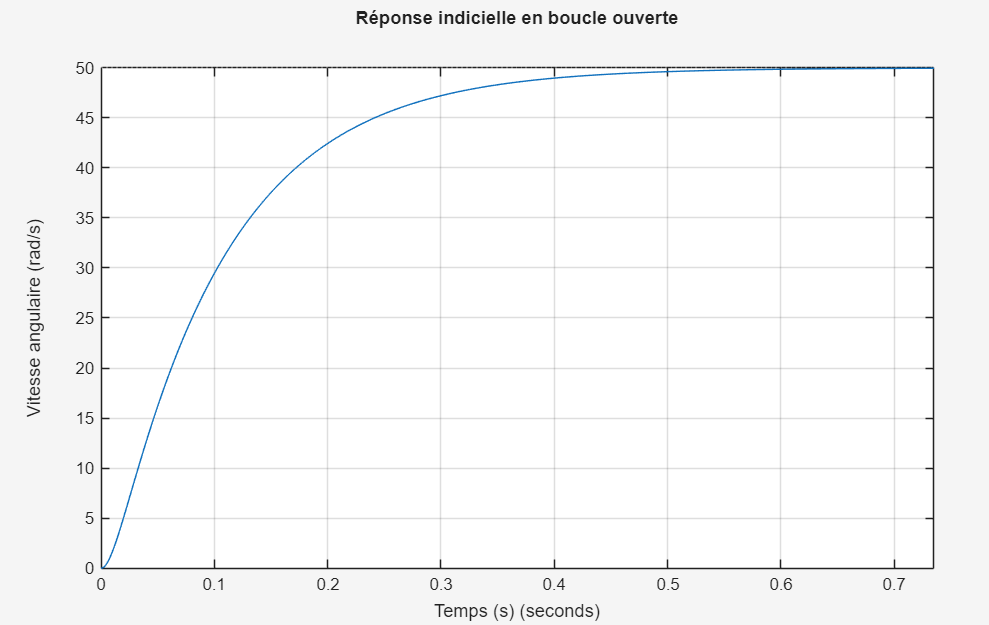
\includegraphics[width=0.7\textwidth]{images/1A_step.png}%%%%%%%%%1A depuis MATLAB, 1A2 depuis simulink
\caption{Réponse indicielle du système en boucle ouverte.}
\end{figure}

La réponse indicielle montre une montée progressive vers la valeur statique de 50~rad/s pour une entrée unitaire de 1~V. Le système est stable et ne présente pas de dépassement en boucle ouverte, ce qui est cohérent avec un système du premier ordre dominant (constante de temps $T_3 = 0.1\ \mathrm{s}$ nettement plus grande que $T_1$ et $T_2$).

% -------------------------------------------------
\subsection{Question B: Tension d'entrée pour une sortie à 50~rad/s}

En régime permanent, boucle ouverte, le gain statique vaut
\begin{equation}
    G(s) = \frac{Y(s)}{U(s)}
\end{equation}
et lorsque t tends vers l'infini, on a :
\begin{equation}
    \lim_{s \to 0} G(s) = K_s
\end{equation}
 $K_s = 50\ \mathrm{rad \cdot s^{-1} / V}$. Pour obtenir une sortie stabilisée à 50~rad/s, il faut donc une entrée de :

\begin{equation}
U_{entree} = \frac{50\ \mathrm{rad/s}}{K_s} = \frac{50}{50} = 1\ \mathrm{V}
\end{equation}

Une tension d'entrée de \textbf{1~V} permet au système de se stabiliser à 50~rad/s en régime permanent.

% -------------------------------------------------
\subsection{Question C: Dimensionnement du gain $K_P$ pour une réponse sans dépassement}

Pour dimensionner $K_P$, on utilise le diagramme de Bode grâce à control system designer
 en boucle fermée $G_{cf}(s) = K_P \cdot G_s(s)$. 

D'après l'annexe 6.A, pour un dépassement nul,
le rapport w_c / w_1 doit être suppérieur à 4.
On regarde la fréquence de coupure w_c sur le diagramme de 
baude qui ici correspond a 100. il nous faut donc un w_1 à 25 
rad/s qui va être obtenue en bougeant la courbe d'amplitude 
jusqu'a avoir une fréquence de coupure de 25 rad/s.
Cela nous donne un gain de $K_P \approx 0.0555$. donnée directement par le bloc C du control system designer.


\begin{figure}[H]
\centering
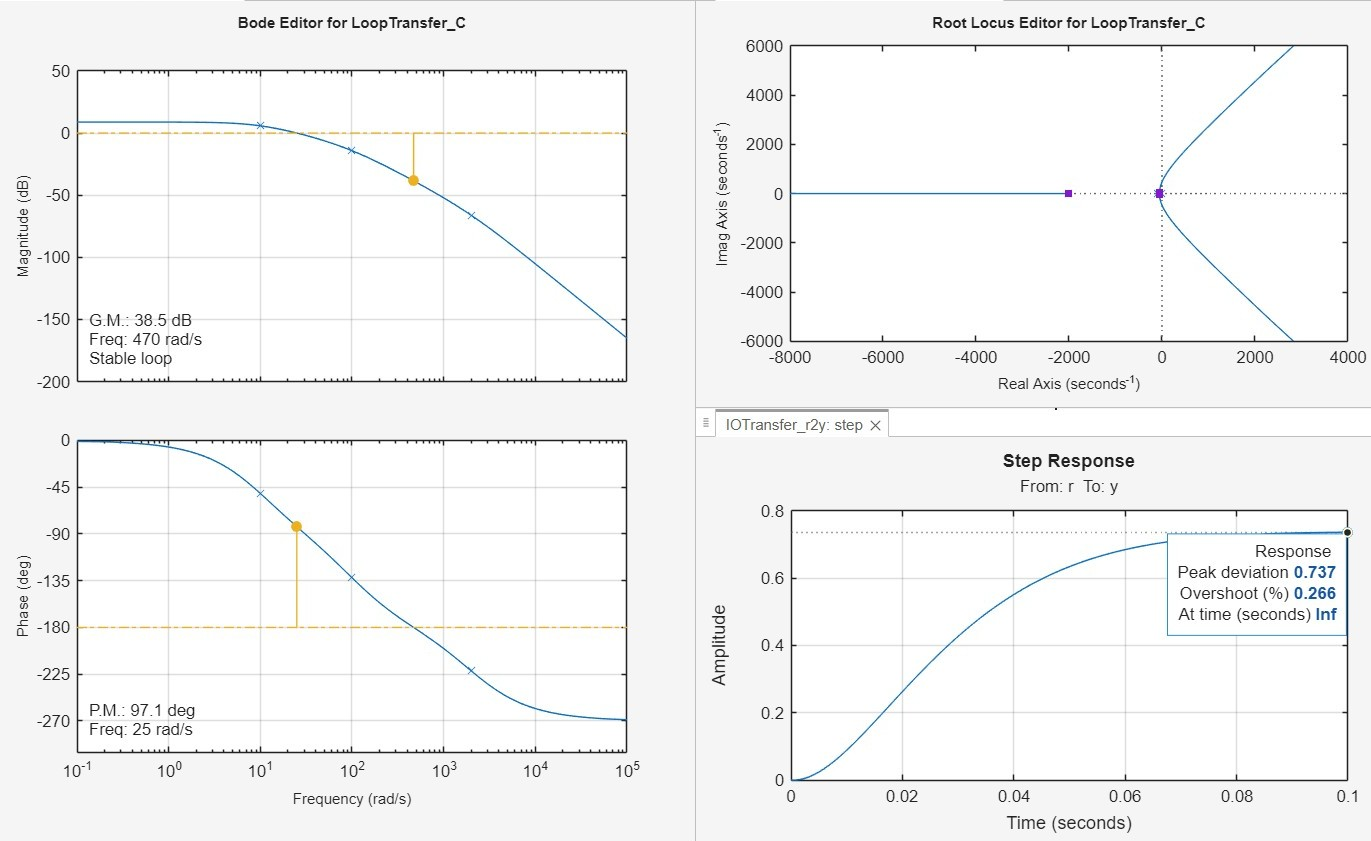
\includegraphics[width=1\textwidth]{images/1C_bode.jpg}
\caption{Diagramme de Bode de $G_s(s)$ avec identification de la fréquence de coupure pour $\varphi_m = 70°$.}
\end{figure}

% -------------------------------------------------
\subsection{Question D: Correction du gain statique}

on peut voir grâce à la step responde du control system designer que le gain statique de la boucle fermée est égal à 0.737.

Ce gain est inférieur à 1 : il existe une erreur statique. Pour que la sortie atteigne la valeur de consigne, il faut appliquer un gain d'entrée $K_{entrée}$ tel que :

\begin{equation}
K_{entrée} = 1/ output\_gain = 1/0.737 \approx 1.36
\end{equation}

Ce gain d'entrée $K_{entrée}$ est placé en amont du système asservi afin de corriger l'erreur de gain statique induite par la boucle fermée.

% -------------------------------------------------
\subsection{Question E: Comparaison boucle ouverte vs boucle fermée}

Les deux systèmes sont simulés en parallèle dans Simulink avec la même entrée en échelon :

\begin{itemize}
\item Système en boucle ouverte : $G_s(s)$ seul, entrée 1~V.
\item Système asservi : boucle fermée avec $K_P$ et correction $K_{entrée}$, consigne 50~rad/s.
\end{itemize}

\begin{figure}[H]
\centering
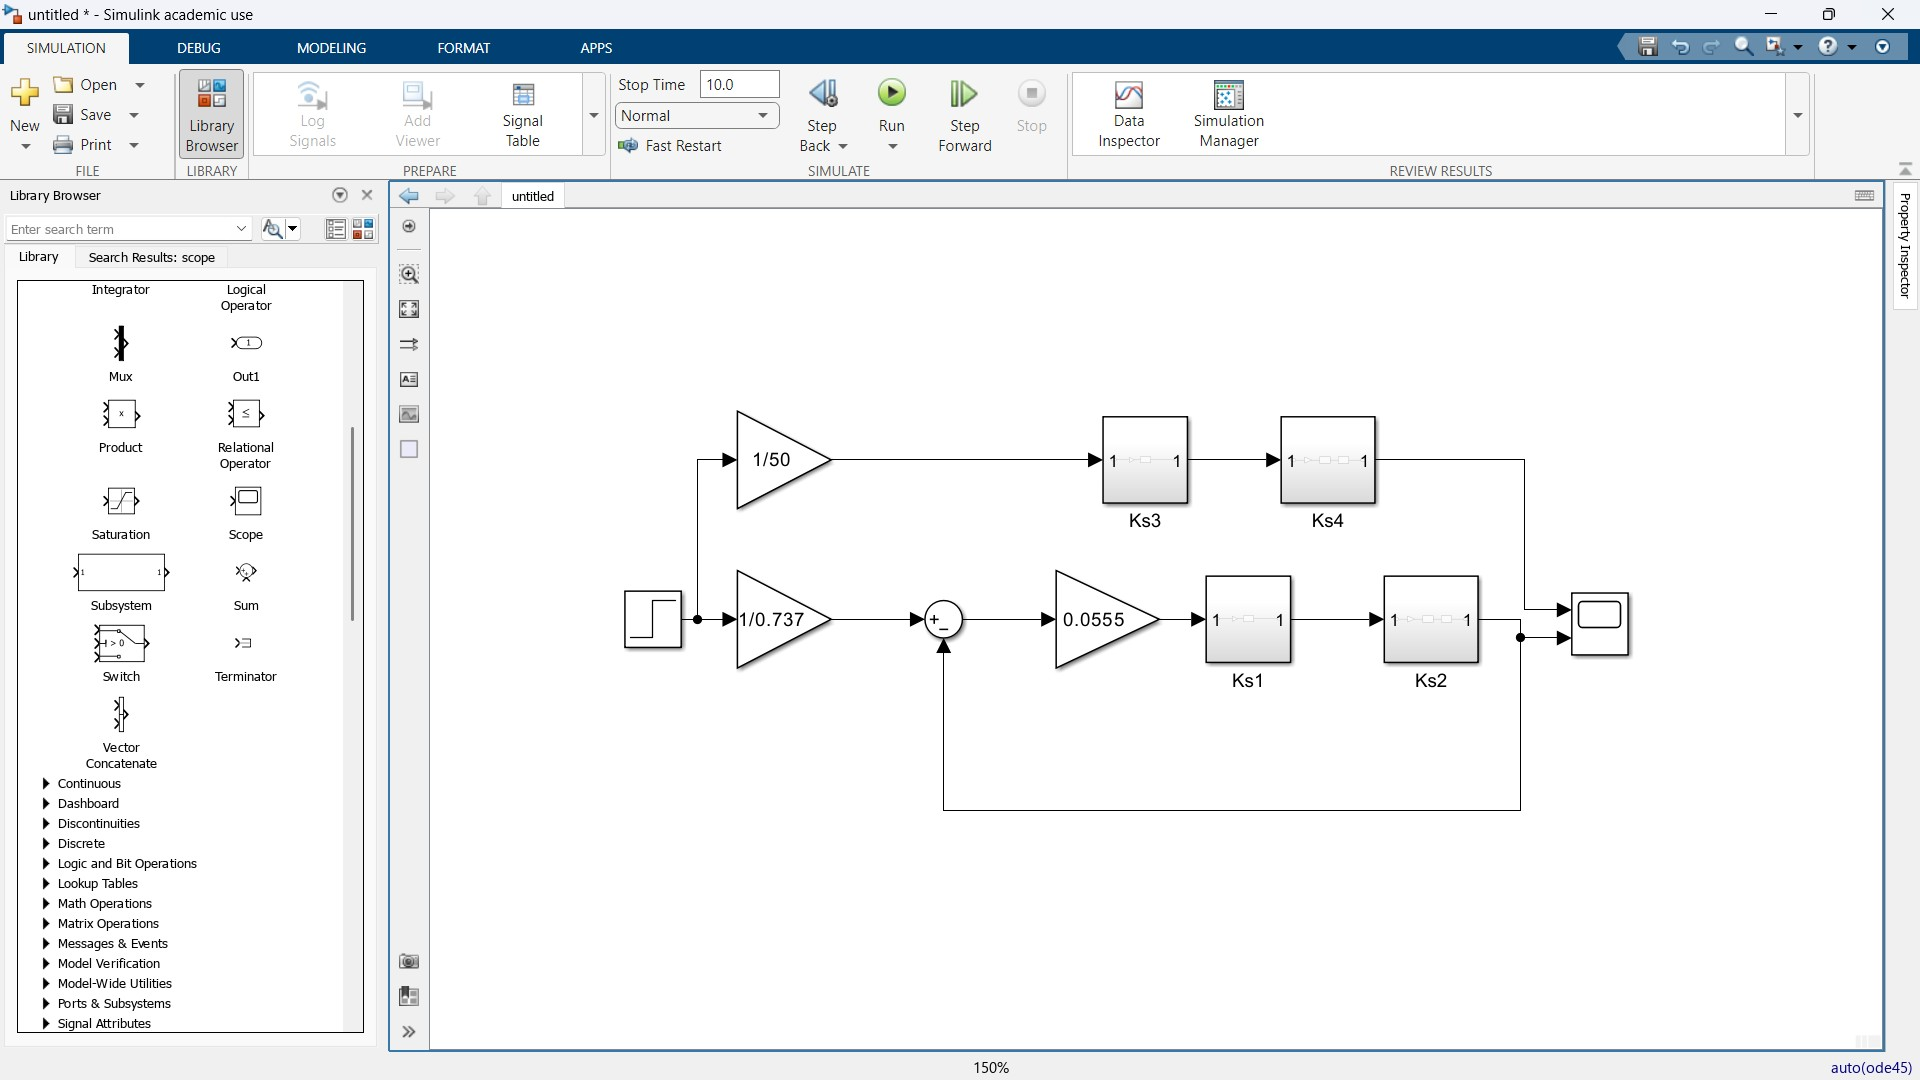
\includegraphics[width=0.75\textwidth]{images/1E_sys.jpg}
\caption{Schéma Simulink comparant les systèmes en boucle ouverte et en boucle fermée.}
\end{figure}

\begin{figure}[H]
\centering
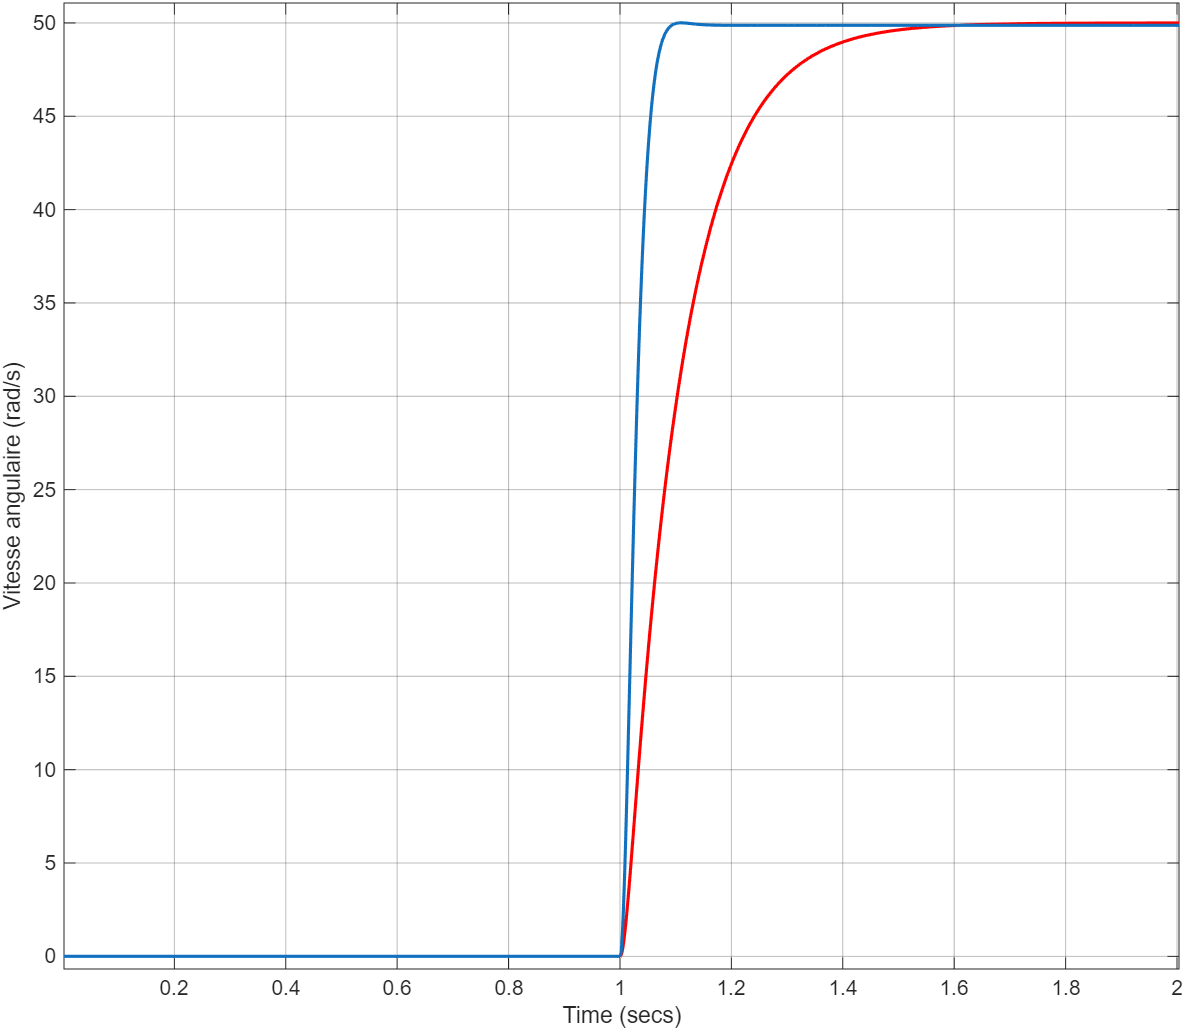
\includegraphics[width=0.75\textwidth]{images/1E_graph.png}
\caption{Comparaison des réponses en boucle ouverte et en boucle fermée (avec $K_P$ et $K_{entrée}$).}
\end{figure}

Le système en boucle fermée est nettement plus rapide que le 
système en boucle ouverte : L'ajout 
du gain d'entrée $K_{entrée}$ assure que la sortie atteint 
bien la consigne de 50~rad/s en régime permanent. 
Le dépassement est nul, conformément à la marge de phase 
dimensionnée.

% -------------------------------------------------
\subsection{Question F: Effet d'une perturbation}

Une perturbation de $1\ \mathrm{mN \cdot m}$ est introduite dans la simulation à $t = 1\ \mathrm{s}$. Elle agit en aval du premier bloc $\frac{K_{s1}}{1 + sT_1}$, directement sur l'entrée du bloc $K_{s2}$.

\begin{figure}[H]
\centering
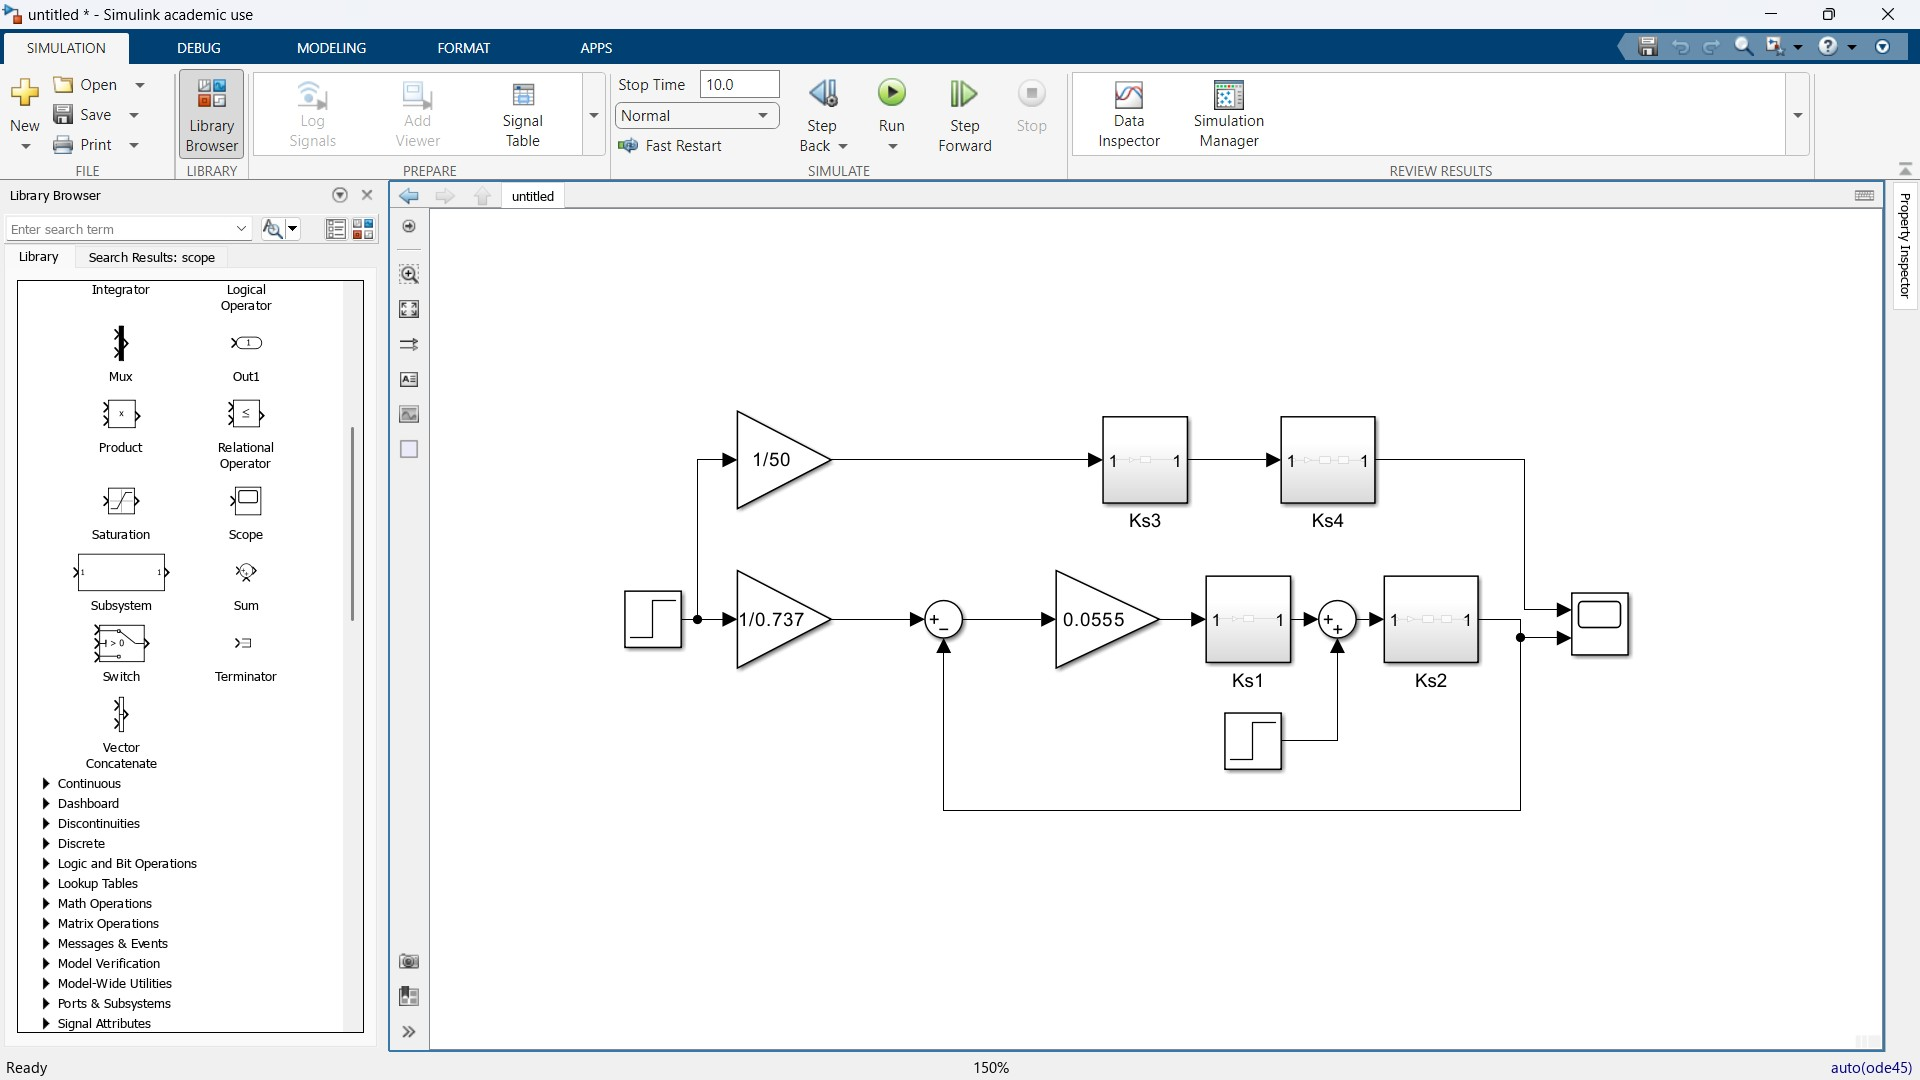
\includegraphics[width=0.75\textwidth]{images/1F_sys.jpg}
\caption{Réponse du système asservi avec régulateur P en présence d'une perturbation de $1\ \mathrm{mN \cdot m}$ à $t = 1\ \mathrm{s}$.}
\end{figure}

L'introduction de la perturbation provoque une déviation permanente de la sortie par rapport à la consigne. Le régulateur proportionnel seul ne peut pas rejeter une perturbation constante : il subsiste une erreur statique résiduelle due à la perturbation. Cette erreur vaut :
\begin{figure}[H]
\centering
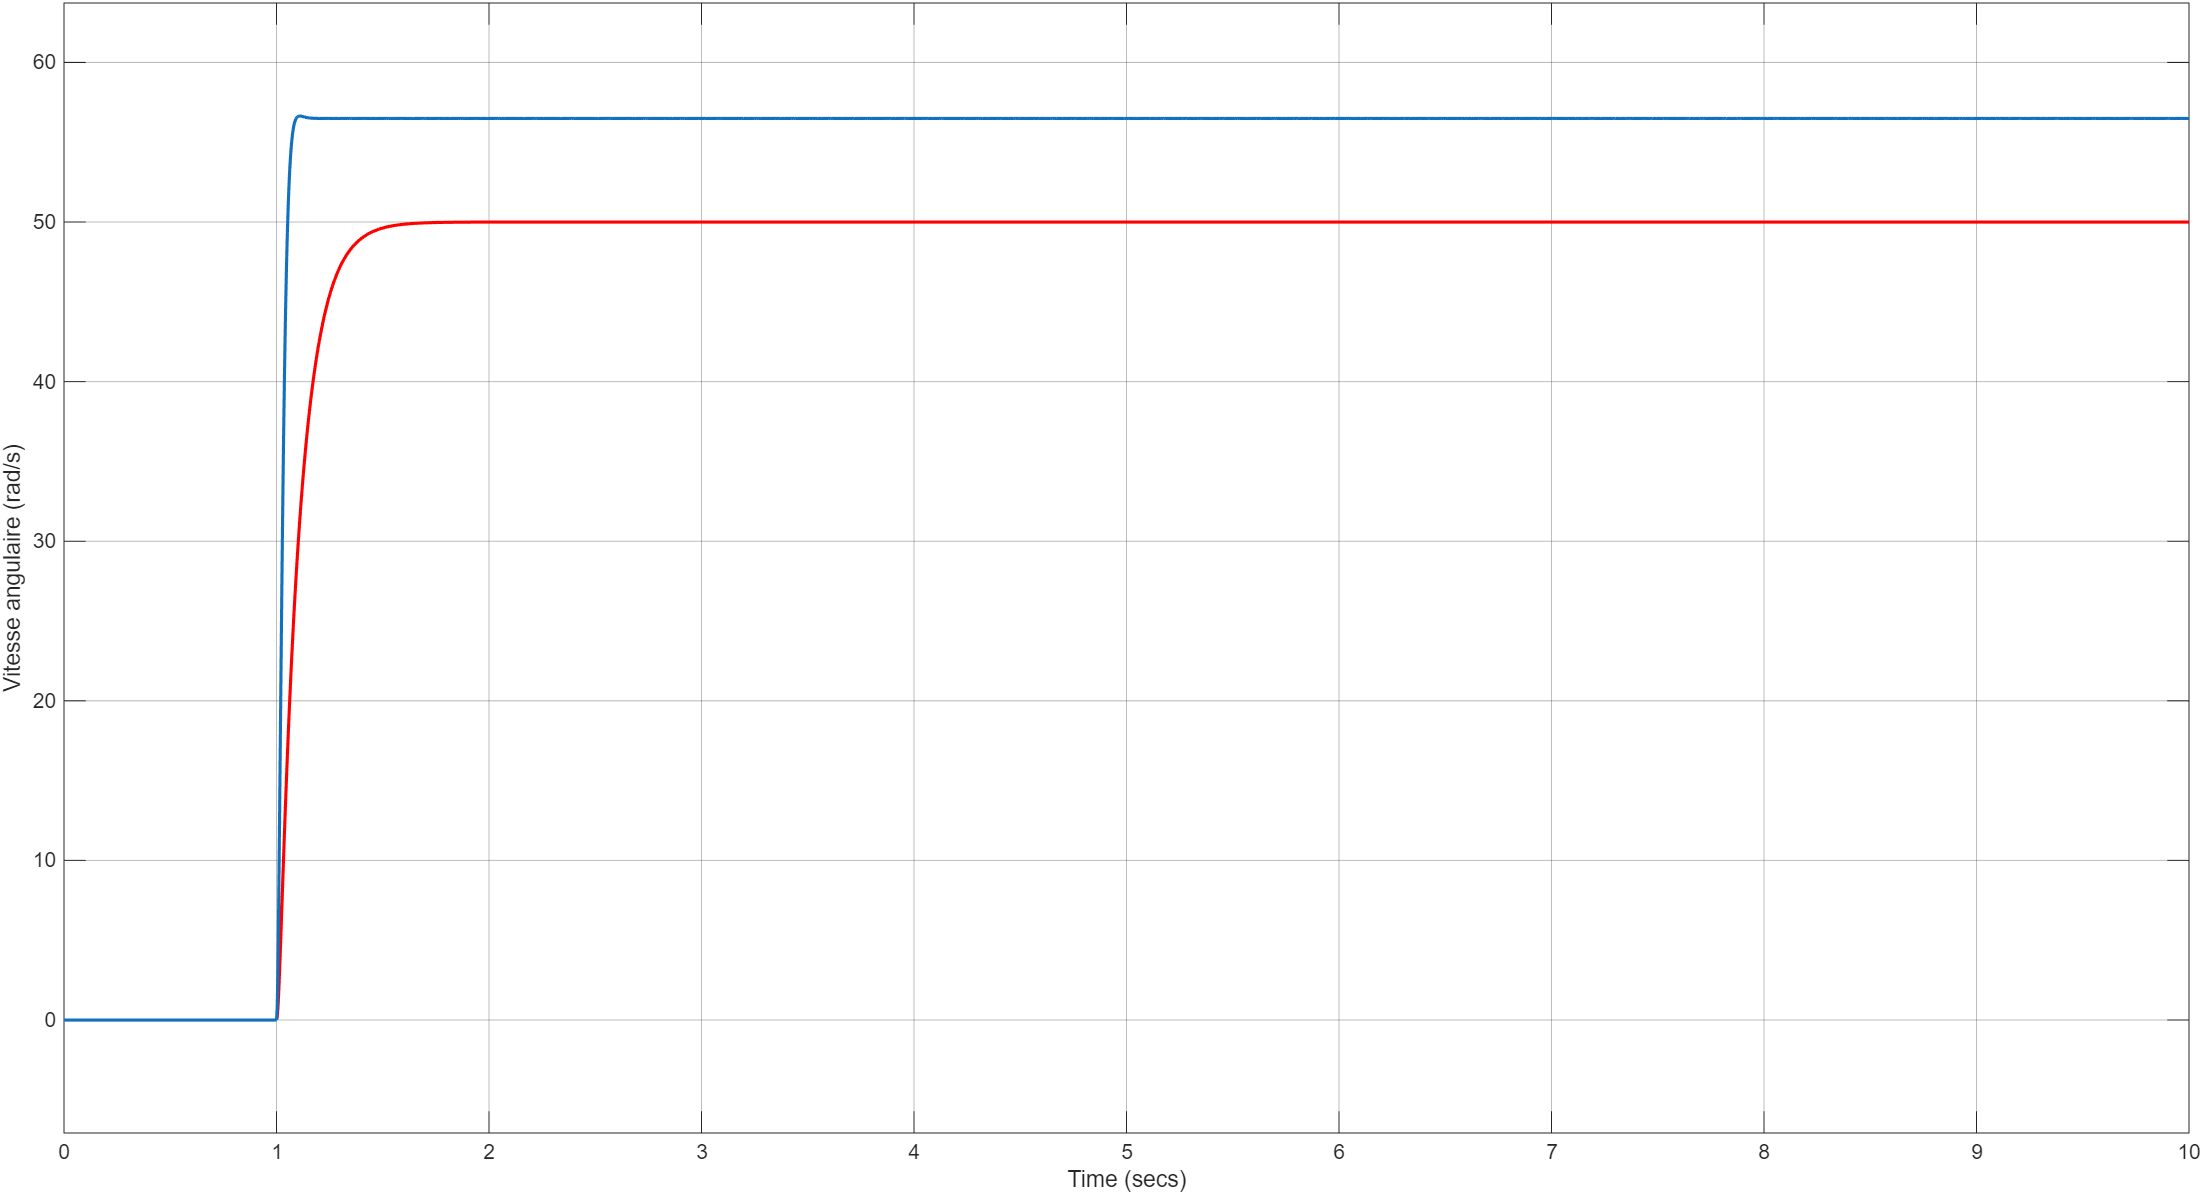
\includegraphics[width=0.75\textwidth]{images/1F_graph.png}
\caption{réponse}
\end{figure}
Le régulateur P est insuffisant pour assurer un rejet total des perturbations constantes.

% -------------------------------------------------
\subsection{Question G: Diagramme de Bode de $G_0(s) = G_R(s) \cdot G_s(s)$}

Avec $G_R(s) = K_P$, le diagramme de Bode de la boucle ouverte $G_0(s) = K_P \cdot G_s(s)$ est tracé dans Control System Designer.

\begin{figure}[H]
\centering
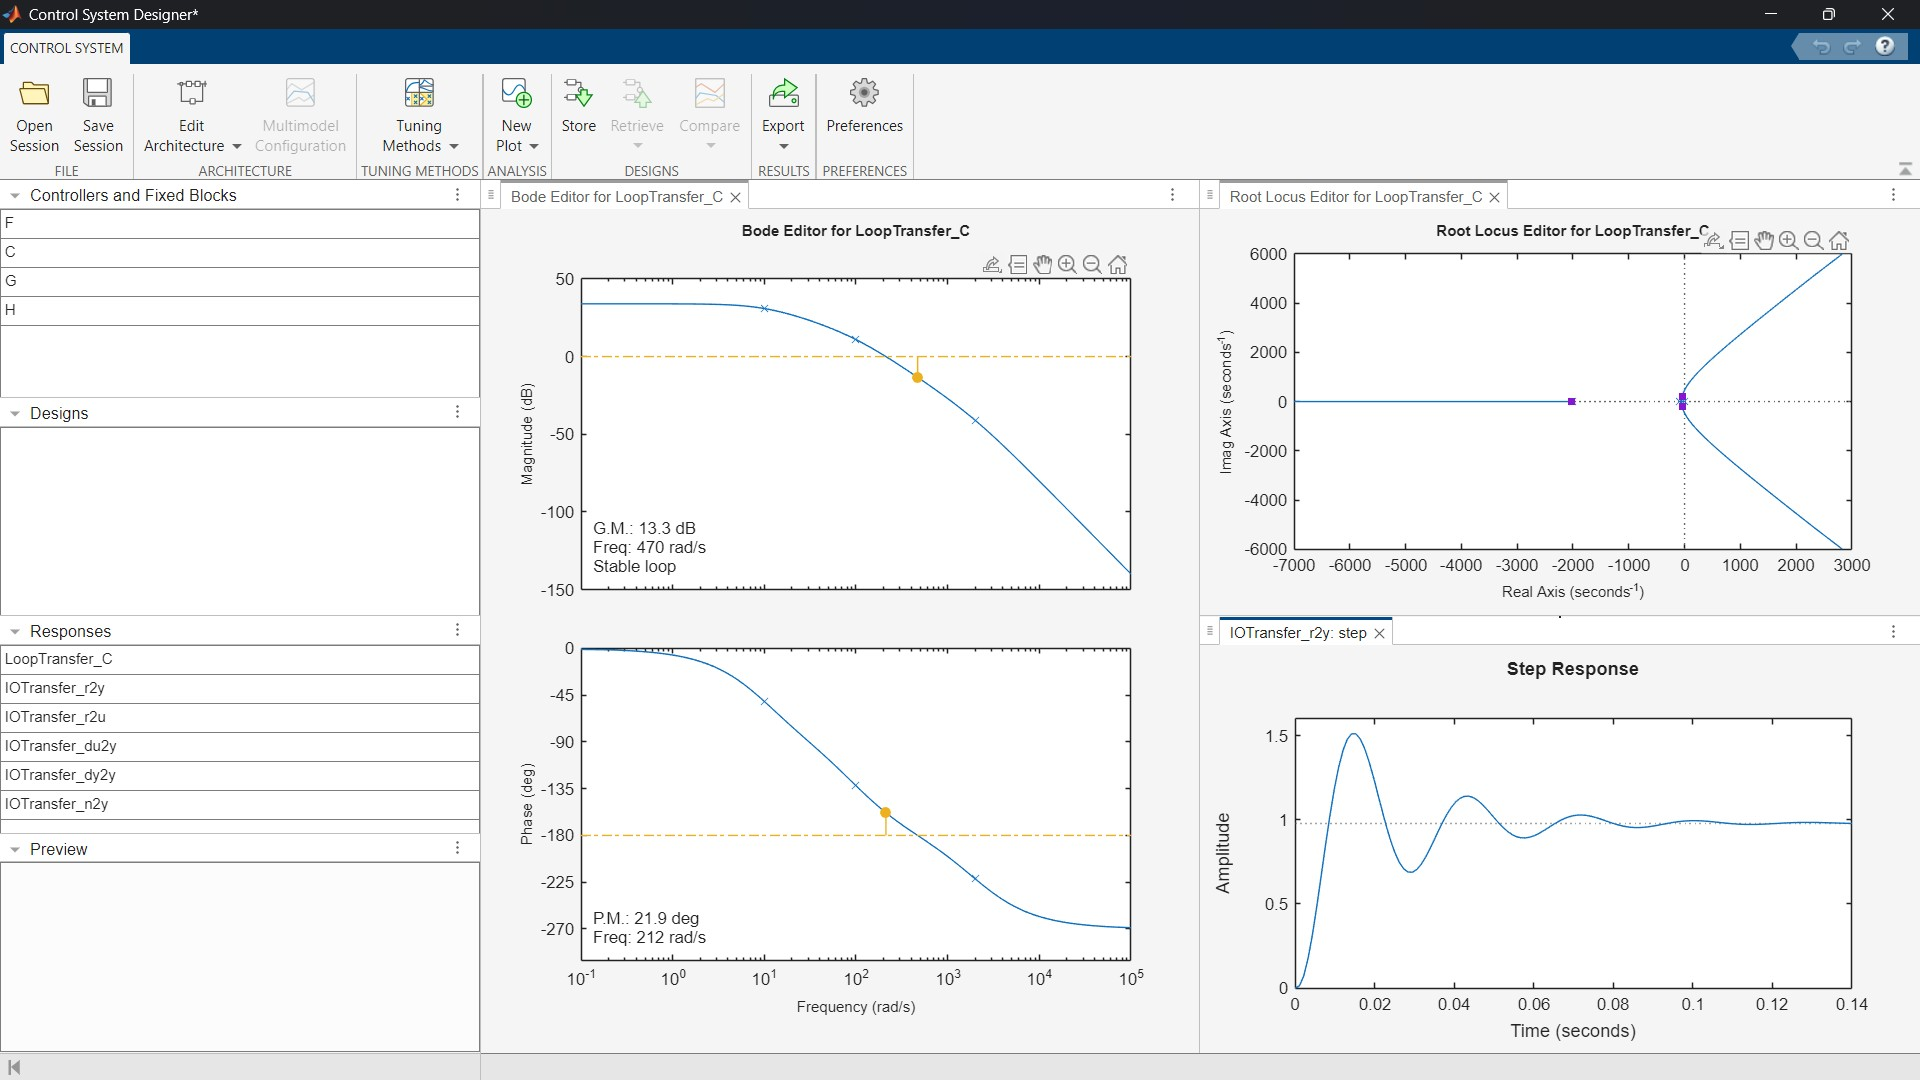
\includegraphics[width=0.75\textwidth]{images/1G_Bode.jpg}
\caption{Diagramme de Bode de $G_0(s) = K_P \cdot G_s(s)$ avec régulateur P.}
\end{figure}

En comparant avec le schéma 6.12 du polycopié (diagramme de Bode idéal d'une boucle ouverte bien dimensionnée), on constate que la pente du diagramme de baude en amplitude commence a -1 et non pas à 0. pour commencer directement à -1 nous allons ajouter un intégrateur.

% -------------------------------------------------
\subsection{Question H: Correction de l'effet de la perturbation}

L'effet indésirable observé au point F (erreur statique résiduelle due à la perturbation) est corrigé par l'ajout d'un \textbf{terme intégrateur} au régulateur. Un régulateur PI (proportionnel-intégral) permet d'annuler l'erreur statique en régime permanent face à toute perturbation constante, car l'intégrateur accumule l'erreur jusqu'à ce qu'elle soit nulle.

\begin{figure}[H]
\centering
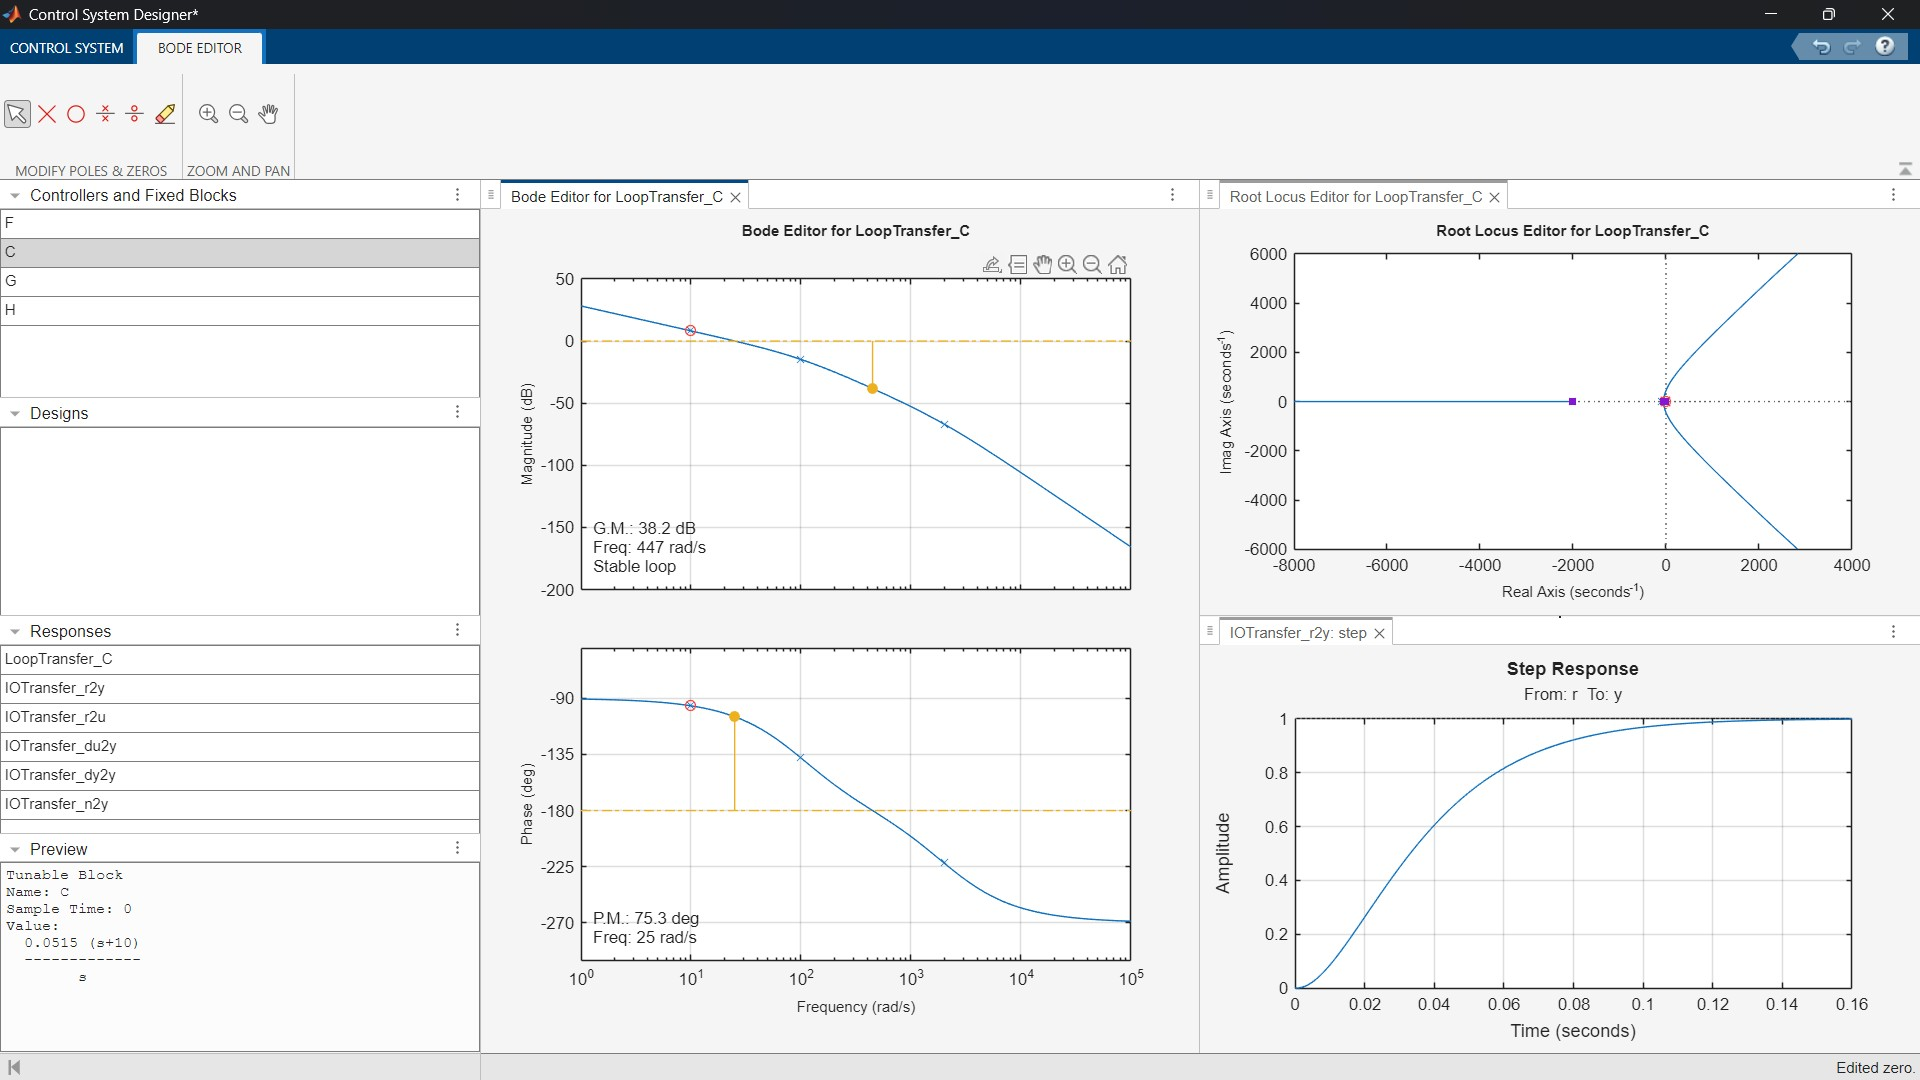
\includegraphics[width=0.75\textwidth]{images/1H_Bode.jpg}
\caption{diagramme PI}
\end{figure}

Le lien avec le point G est direct : l'ajout d'un intégrateur dans $G_R(s)$ ajoute un pôle en $s = 0$, ce qui fait basculer la pente de la boucle ouverte à $-40\ \mathrm{dB/décade}$ en basse fréquence.

% -------------------------------------------------
\subsection{Question I: Implémentation du régulateur PI dans Simulink}

Le régulateur PI s'écrit sous la forme :

\begin{equation}
G_R(s) = K_P \cdot \frac{1 + T_n \cdot s}{T_i \cdot s}
\end{equation}

la valeur de l'intégrateur I est donnée par l'ajout d'un intégrateur sur le diagramme de baude sur control system designer.


\begin{figure}[H]
\centering
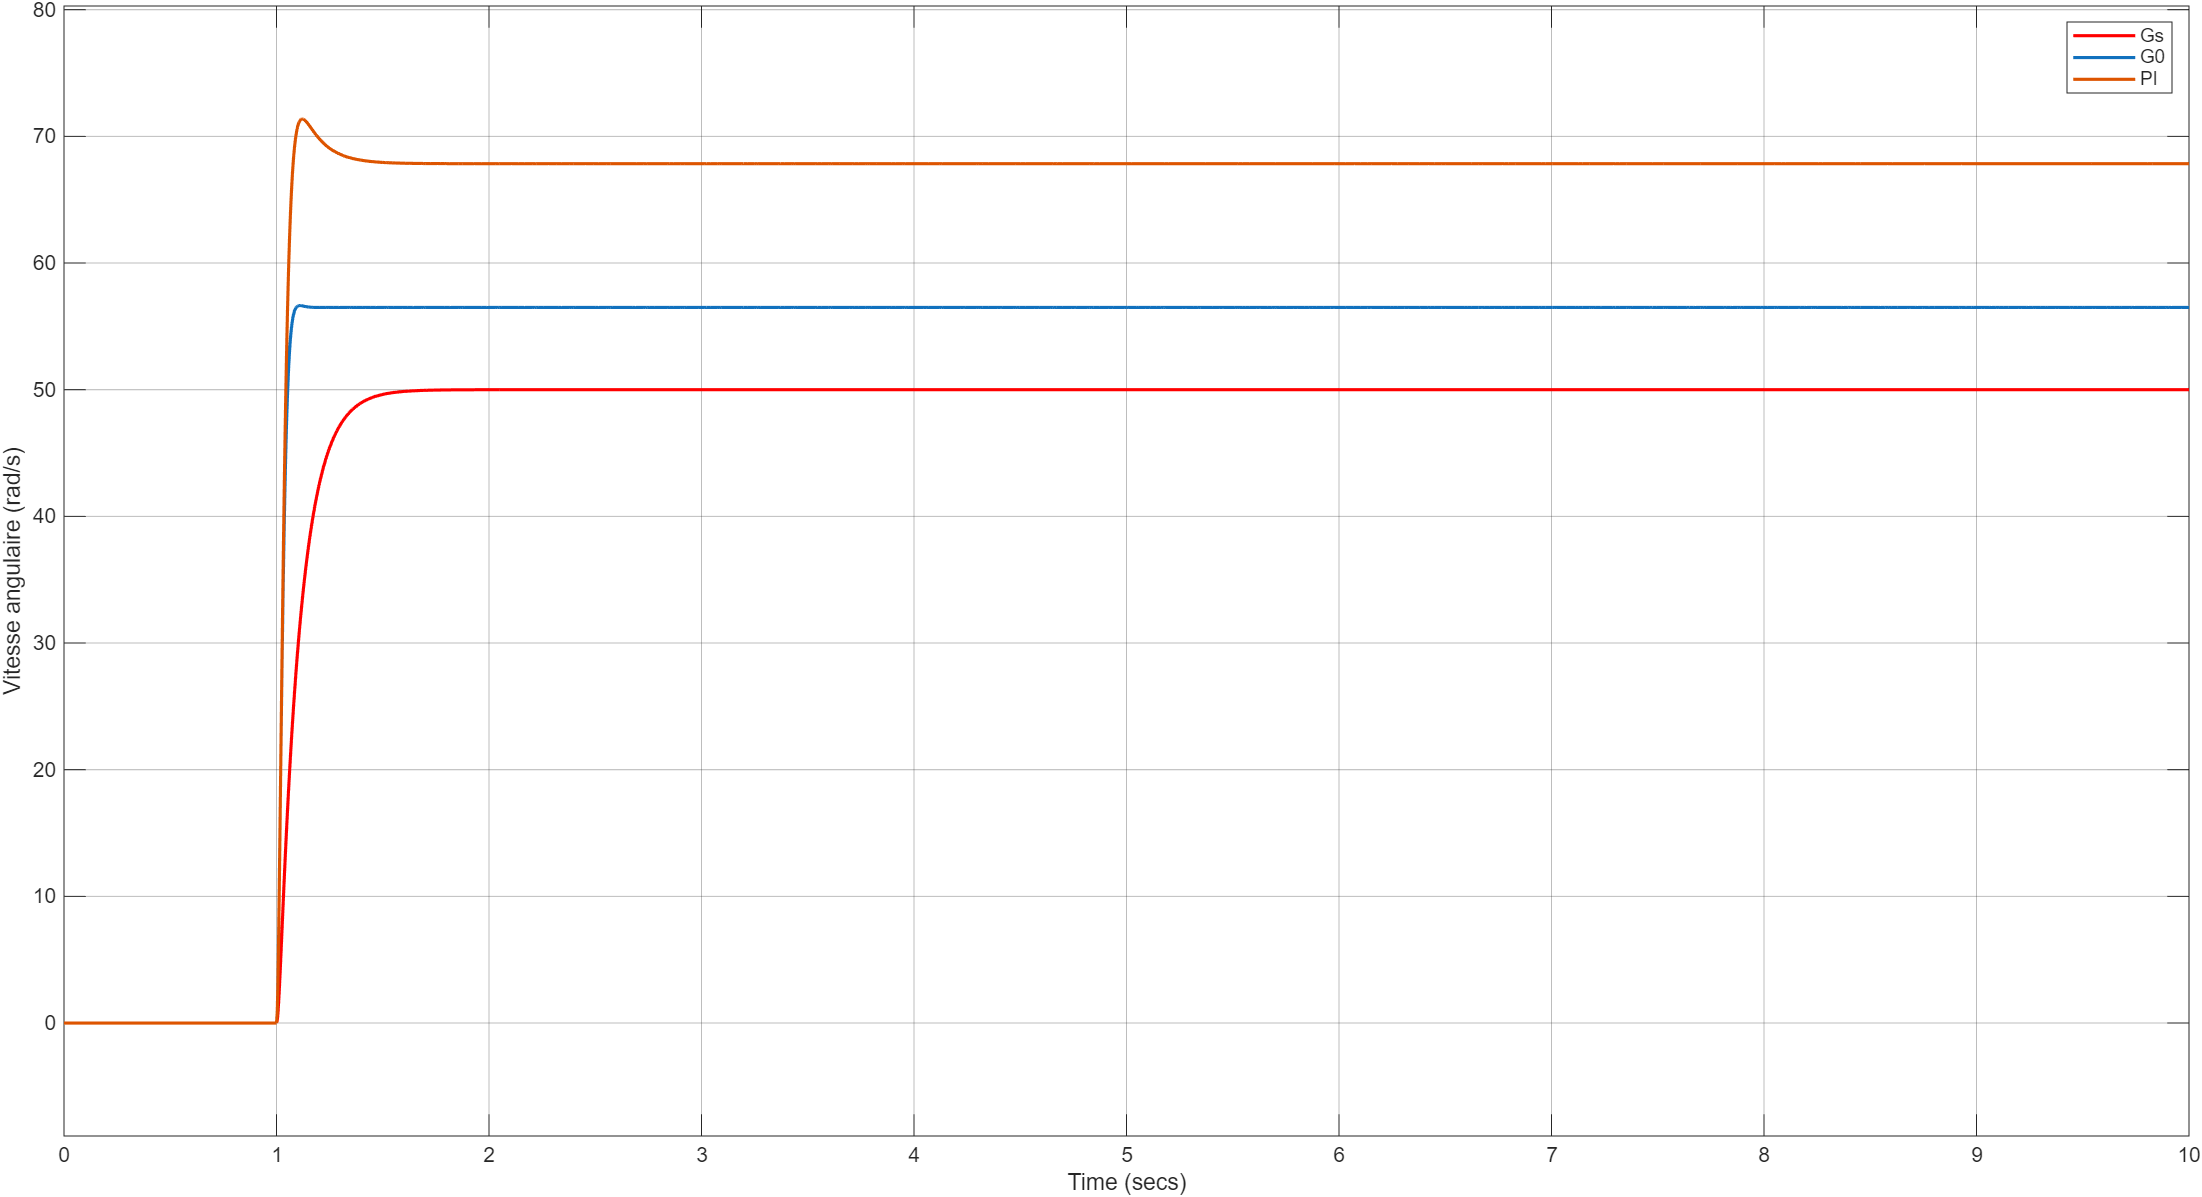
\includegraphics[width=0.75\textwidth]{images/1I_graph.png}
\caption{a}
\end{figure}

Avec le régulateur PI, la sortie revient à la consigne après l'application de la perturbation. L'erreur statique est bien nulle en régime permanent.

% -------------------------------------------------
\subsection{Question J: Amélioration de la dynamique -- régulateur PID}

La dynamique peut encore être améliorée en ajoutant un \textbf{terme dérivateur} au régulateur PI, ce qui donne un régulateur \textbf{PID}. Le terme dérivateur permet d'augmenter la fréquence de coupure de la boucle ouverte, c'est-à-dire d'accélérer la réponse du système tout en maintenant une marge de phase suffisante.

Le principe consiste à compenser un second pôle du système (par exemple $T_2 = 0.01\ \mathrm{s}$) avec le zéro apporté par le terme dérivateur :

\begin{equation}
G_R(s) = K_P * \frac{(1+sTn)(1+sTv)}{s*Ti}
\end{equation}


\begin{figure}[H]
\centering
\includegraphics[width=0.75\textwidth]{images/1J_PID_comparaison.png}
\caption{Comparaison des réponses avec régulateurs P, PI et PID. Le PID offre la dynamique la plus rapide avec un rejet de perturbation optimal.}
\end{figure}

Le régulateur PID permet d'obtenir une réponse plus rapide que le PI, avec un dépassement maîtrisé. La compensation de deux pôles du système libère de la marge de phase, ce qui permet d'augmenter le gain et donc la fréquence de coupure.

% -------------------------------------------------
\subsection{Question K: Diagramme de Bode de $G_0(s)$ avec régulateur PID}

Le diagramme de Bode de $G_0(s) = G_{PID}(s) \cdot G_s(s)$ est tracé dans Control System Designer.

\begin{figure}[H]
\centering
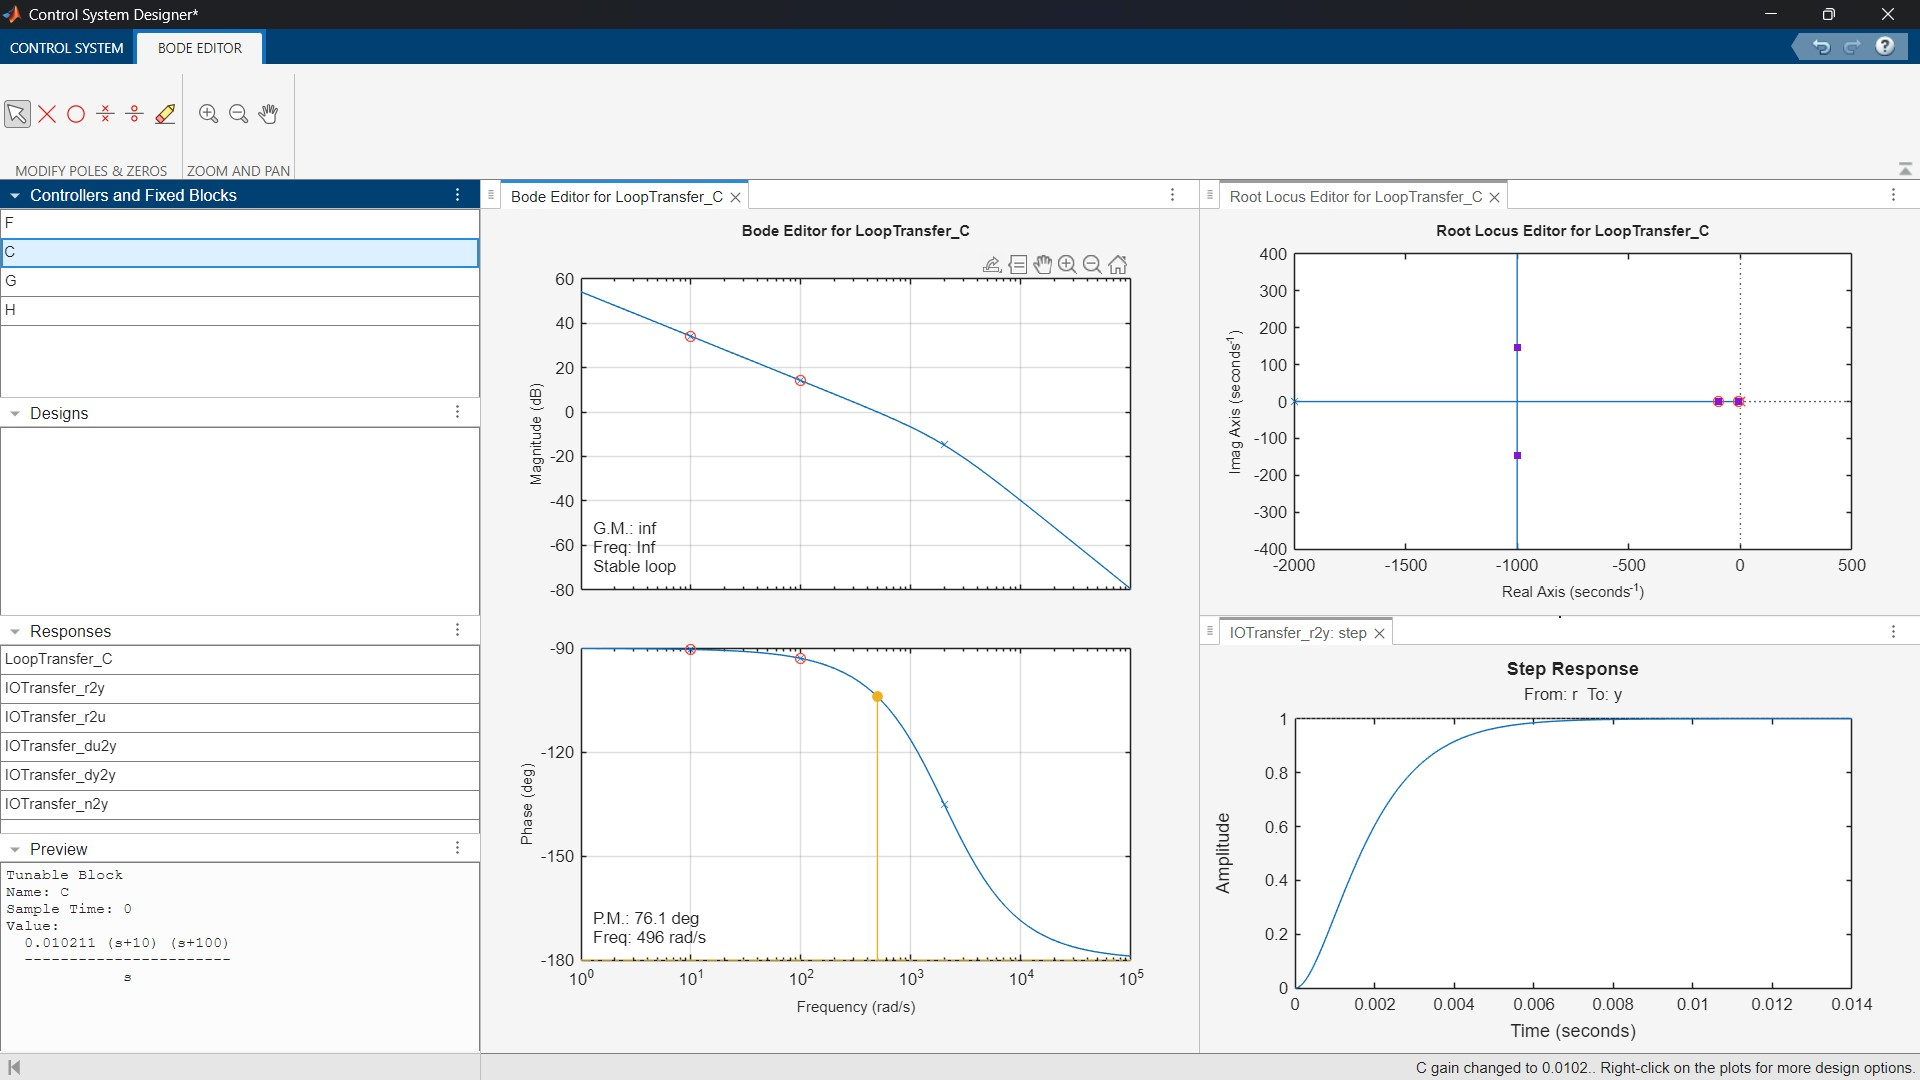
\includegraphics[width=0.75\textwidth]{images/1K2_bode.jpg}
\caption{Diagramme de Bode de $G_0(s)$ avec régulateur PID.}
\end{figure}

En comparant avec le schéma 6.12 du polycopié :

% =================================================
\section{Conclusion}

Ce laboratoire a permis de comprendre le rôle des différents types de régulateurs dans un système asservi. Le régulateur proportionnel améliore la rapidité du système et permet de dimensionner une marge de phase satisfaisante, mais il ne peut pas rejeter les perturbations constantes. L'ajout d'un terme intégrateur (régulateur PI) permet d'éliminer l'erreur statique due aux perturbations, au prix d'une légère réduction de la dynamique. Enfin, l'ajout du terme dérivateur (régulateur PID) permet de compenser les pôles lents du système et d'améliorer significativement la rapidité de la réponse.

La méthode de dimensionnement par le diagramme de Bode s'est révélée efficace : elle permet de choisir le gain de manière rigoureuse en fixant une marge de phase cible, et d'interpréter directement l'effet de chaque terme du régulateur sur le comportement fréquentiel de la boucle ouverte.

\section*{Annexes}
\begin{figure}[H]
\centering
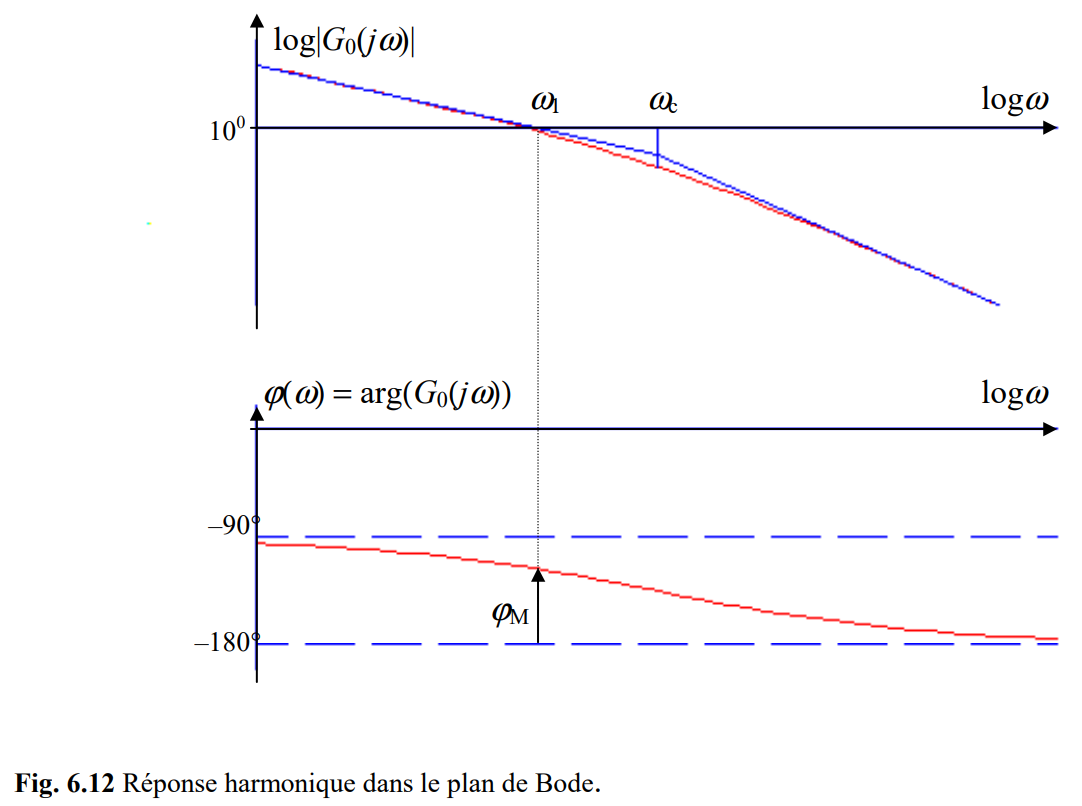
\includegraphics[width=0.75\textwidth]{images/schema_6.12.png}
\caption{Schéma de référence du polycopié 6.12.}
\end{figure}

\end{document}